\documentclass[conference]{IEEEtran}
\IEEEoverridecommandlockouts
\usepackage{cite}
\usepackage{amsmath,amssymb,amsfonts}
\usepackage{algorithmic}
\usepackage{graphicx}
\usepackage{textcomp}
\usepackage{xcolor}
\usepackage{url}
\usepackage{array}
\usepackage{tikz}
\usetikzlibrary{arrows.meta,positioning,fit,calc}
\hyphenpenalty=10000
\exhyphenpenalty=10000
\emergencystretch=1.5em
\raggedbottom
\makeatletter
\newcommand{\authorflushleft}{\end{@IEEEauthorhalign}\hskip 0pt plus -1fill\begin{@IEEEauthorhalign}}
\newcommand{\linebreakand}{\end{@IEEEauthorhalign}\hfill\mbox{}\par\mbox{}\hfill\begin{@IEEEauthorhalign}}
\makeatother
\def\BibTeX{{\rm B\kern-.05em{\sc i\kern-.025em b}\kern-.08em
    T\kern-.1667em\lower.7ex\hbox{E}\kern-.125emX}}

% ---------------------------------------------------------------------
\newcommand{\embmodel}{\texttt{snowflake\allowbreak-arctic\allowbreak-embed\allowbreak-xs}}
\newcommand{\embdim}{384}
\newcommand{\rerankmodel}{\texttt{ms\allowbreak-marco\allowbreak-MiniLM\allowbreak-L\allowbreak-6\allowbreak-v2}}
\newcommand{\llmname}{GPT\nobreakdash-6 Luna}
% ---------------------------------------------------------------------

\tikzset{
  box/.style={draw, rounded corners=2pt, align=center, font=\footnotesize,
              minimum height=6mm, inner sep=3pt, fill=white},
  store/.style={box, fill=gray!12},
  llm/.style={box, fill=gray!28, font=\footnotesize\bfseries},
  arr/.style={-{Stealth[length=2mm]}, semithick},
  grp/.style={draw, dashed, rounded corners=3pt, inner sep=4pt}
}

\begin{document}

\title{E.C.H.O: An Intent Aware Personal Memory System for Unified Search Across Email, Web, and Video History}

\author{\IEEEauthorblockN{1\textsuperscript{st} Arjun Sai N}
\IEEEauthorblockA{\textit{Dept. of Computer Science} \\
\textit{and Engineering} \\
\textit{PES University}\\
Bengaluru, India}
\and
\IEEEauthorblockN{2\textsuperscript{nd} Mohammed Mir Fazlai Ali}
\IEEEauthorblockA{\textit{Dept. of Computer Science} \\
\textit{and Engineering} \\
\textit{PES University}\\
Bengaluru, India}
\and
\IEEEauthorblockN{3\textsuperscript{rd} Mohammed Shehzaad Khan}
\IEEEauthorblockA{\textit{Dept. of Computer Science} \\
\textit{and Engineering} \\
\textit{PES University}\\
Bengaluru, India}
\linebreakand
\IEEEauthorblockN{4\textsuperscript{th} Mrigank Jain}
\IEEEauthorblockA{\textit{Dept. of Computer Science} \\
\textit{and Engineering} \\
\textit{PES University}\\
Bengaluru, India}
\and
\IEEEauthorblockN{5\textsuperscript{th} Mannuru Shalima Sulthana}
\IEEEauthorblockA{\textit{Dept. of Computer Science} \\
\textit{and AIML} \\
\textit{PES University}\\
Bengaluru, India}
}

\maketitle

\begin{abstract}
Take one interview. The invitation sits in Gmail, the articles read to prepare for it sit in Chrome's history, and the tutorials sit in YouTube's watch history. Each app has its own search box, and none of them knows what the other two hold. We built E.C.H.O (Efficient Contextualized History Orchestrator) to fix this for a single user. It brings Gmail, Chrome, and YouTube activity into one store on the user's laptop and answers questions about it in plain language. What gets stored depends on the source. All mail is kept, except what Gmail has already put in spam or trash, but a page or a video is kept only when foreground time, scrolling, watch time, or a return visit shows that the user paid attention to it. In the background, a worker cleans each item and pulls text out of its attachments. Every item is embedded too, and it lands in one of 5 broad categories. Now when a question comes, a language model plans the search, but the search itself is plain code, and all of it sits behind one tool only. Inside that tool keyword search and vector search run side by side, reciprocal rank fusion makes one list out of the two, and a local cross encoder does the final ordering, but if the results come back weak the search gets widened first. Usually it is 2 model calls for a question, and the code stops it at 6. The database rows and the whole store, those the model never sees, it gets the question and limited excerpts and nothing more. The wellbeing module, it shows where the time went without judging it, and it files items into the user's own goals by itself only when two signals agree, everything else waits for the user. We tested on 119 items, 78 emails, 30 pages and 11 videos, with 38 questions, and 93\% of the relevant items were in the first ten results, with 2.3 model calls and a median of 8.1 seconds per question. The capture rules matched in all 13 clean scripted sessions. One thing we did not expect, semantic search alone ranked better than the full pipeline, because in the questions we checked, the cross encoder gave every candidate a score near zero and the engagement term ended up deciding the order.
\end{abstract}

\begin{IEEEkeywords}
personal information management, intent aware capture, hybrid search, reciprocal rank fusion, retrieval augmented generation, tool calling agents, local first software, digital wellbeing
\end{IEEEkeywords}

% ---------------------------------------------------------------------
\section{Introduction}
% ---------------------------------------------------------------------
In placement season at PES University this happens a lot, a company mails the interview schedule and then for some days the preparation goes on, operating systems articles in Chrome, a few explanations on YouTube, and a week later just before the interview all of it is needed again. By then the email is in Gmail, the videos in YouTube watch history and the articles somewhere in Chrome history, three different places for one interview. Each app searches only its own data, so getting everything back means three separate searches and some guessing about which app holds what.

People have wanted to keep a record of everything they have seen for a long time, so this is an old idea actually. Bush described the memex in 1945 \cite{b1}, and much later Stuff I've Seen \cite{b2} and MyLifeBits \cite{b3} built working stores of a person's mail, pages, and documents. Still, it has not become something people use daily, and noise is a big reason for that. A browser logs every page that opens, stray clicks and tabs closed after two seconds included, and a memory built straight on that log is mostly pages nobody read. Our capture test has exactly this case, a page closed after three seconds, and E.C.H.O is expected to drop it (Section~\ref{sec:eval}). And even a clean memory is hard to search. A search box wants the right keyword, but people do not remember keywords. They remember something like ``the OS material I read after the interview email.''

E.C.H.O deals with each problem at a different point. Noise is handled at capture. A page or a video is stored only if engagement shows that the user actually attended to it, so the stray tab does not reach the database at all. The keyword problem is handled at search time. E.C.H.O searches by meaning as well as by keyword, and a language model turns the user's loose phrasing into concrete searches. Mail, pages, and videos share one data model on the user's laptop, they get enriched in the background, and the user asks about them in natural language. So every answer is built from the stored items, if someone asks about the offer letter the answer comes from that mail and not from what the model remembers, which is retrieval augmented generation \cite{b4}.

We have four contributions in this work, and they are as follows:
\begin{itemize}
\item Capture, where each source has separate rules and the privacy filters run before anything is stored, so sensitive pages lose their text, secret parameters get cut from the addresses, and private work apps keep only the page title. In all 13 clean scripted sessions the stored items matched these rules.
\item Storage, which is one local model, emails, pages and videos all share one central table and the schema has 17 tables. PostgreSQL is the permanent record and Redis is for short lived state. FAISS can be rebuilt from PostgreSQL any time, so even if the index goes nothing is lost. Attachment text gets extracted when the mail arrives, so a PDF can be found as easily as the email it came with.
\item Retrieval, and here we use a bounded agentic loop. Each search is planned and phrased by the model, but running it is the deterministic tool's job, and that tool has hybrid keyword and vector search, rank fusion, cross encoder reranking, and a rule based quality check that widens the weak searches. On average a turn took 2.34 model calls in our test, and the code allows at most 6.
\item Wellbeing, the module reports time, sessions and declared regret, only descriptive, and there is a grouping engine for the user's own goals. There is only one thing, for an item to get filed on its own a rule match has to agree with a neighbor score of at least 0.85, and even that is undone with one click. All other suggestions wait for the user, and at 0.85 no outside item got in during the test.
\end{itemize}

Section~\ref{sec:related} is the related work and Section~\ref{sec:overview} gives an overview, after that Sections IV to VI cover capture, storage, enrichment, retrieval, wellbeing and privacy, then the implementation is in Section~\ref{sec:impl} and Section~\ref{sec:eval} has the results. Finally, Section~\ref{sec:limits} lists the limitations, and Section~\ref{sec:conc} concludes.

% ---------------------------------------------------------------------
\section{Related Work}\label{sec:related}
% ---------------------------------------------------------------------
\subsection{Personal Information Management}
Bush pictured the memex as a desk that keeps a person's books, records, and letters and brings any of them back quickly \cite{b1}. Stuff I've Seen put everything a person had already seen, such as an email, a web page, or a document, under one index, and used the fact that the person had seen it before as a cue for search \cite{b2}. MyLifeBits went further and tried to keep everything that could be captured, in a SQL database \cite{b3}. E.C.H.O wants what these systems wanted, which is to help a person find something again. Where it differs is in what it keeps and what it gives back. MyLifeBits would store the page that was open for three seconds, but E.C.H.O never writes it. Stuff I've Seen returns a list of results, while E.C.H.O returns an answer, with a small pill for each source it used.

\subsection{Retrieval Augmented Generation and Tool Use}
In retrieval augmented generation, a retriever fetches documents and a text generator writes its answer from them \cite{b4}. In E.C.H.O, the retriever is the \texttt{search\_memories} tool and the generator is \llmname{}, and the steps are arranged as a graph built with LangGraph \cite{b5}. ReAct showed that a language model can alternate between reasoning and actions such as search calls, and that grounding each step in tool output reduces invented facts \cite{b13}. We borrow this pattern, but in a deliberately narrow form. The model has exactly one read only tool. Apart from two small local encoders, this tool has no model inside it. Also, the code caps how many rounds the model gets.

\subsection{Hybrid Search and Reranking}
Like an interview mail and a placement email, they mean the same thing so they come close, that is what Sentence BERT \cite{b6} showed, texts get turned into vectors where the cosine similarity follows the meaning. E.C.H.O embeds every item with a small local sentence model \cite{b16} and searches the vectors with FAISS \cite{b8}. For keyword search we use PostgreSQL's own full text search which is built in, it catches the things meaning misses like sender names, domains and channel names. We saw this while testing in July, a question about ``emails from Neon'' was not matching the sender at all, and only after we added senders to the text index did it start matching. The problem is that these two methods score on unrelated scales, so it does not make sense to add their scores directly. Reciprocal rank fusion solves this because it uses just the position of each item in each list \cite{b9}. After fusion, a cross encoder reads the question and a candidate together and scores how well they match. Nogueira and Cho showed that this works well for passage reranking \cite{b10}. Our cross encoder is a compact MiniLM \cite{b7} model, trained on the MS MARCO passage ranking data \cite{b11}.

\subsection{Local First Software}
Kleppmann et al.\ describe local first software, where users own their data and the application works from a copy on their own device \cite{b12}. E.C.H.O follows the same idea, as the database, the vector index, the cache, and both encoders all run on the user's laptop. The hosted language model gets only limited pieces of text.

\subsection{Digital Wellbeing Tools}
Lyngs et al.\ reviewed hundreds of digital self control apps and browser extensions. They found that most of them block, limit, or track usage against a goal \cite{b14}. If someone spent three hours on YouTube, E.C.H.O shows the three hours and that is it, whether it was good or bad the user decides, not E.C.H.O. It shows where the time went, and the user decides which items they regret, with no score and no blocking. We hold the generated text to the same rule. The weekly reflection is checked for judging phrases before it is shown, and if it fails that check, the user sees plain numbers instead (Section~\ref{sec:wba}).

% ---------------------------------------------------------------------
\section{System Overview}\label{sec:overview}
% ---------------------------------------------------------------------
Fig.~\ref{fig:arch} shows the main parts of the system. First, data comes in through three connectors. The Gmail connector reads mail through the Gmail API with OAuth, and it asks only for the changes since its last check. The Chrome extension follows desktop browsing and YouTube playback. It runs on the whole YouTube site and not only on \texttt{/watch} pages. YouTube switches videos without reloading the page, so an earlier version of the extension missed the videos that a user opened from inside the site. The YouTube connector then adds each video's details from the YouTube Data API. Next, all connectors send their items to one FastAPI gateway, and there the storage engine writes each item in a single transaction and skips anything already stored.

The work is then split across three stores. PostgreSQL keeps the permanent record of all items. FAISS keeps the embedding vectors, and we treat it as something that can always be rebuilt. We learned this in July, when a corrupted metadata file left semantic search silently returning nothing, and we rebuilt the index from the text stored in PostgreSQL. Keeping the stored text identical to the embedded text is what makes such a rebuild exact. And Redis is used for short lived state, revisit flags, cached attachment text, reminder state, the capture settings, all of this on the user's laptop itself.

On top of the stores there are three modules. The enrichment worker (ENP) prepares new items in the background, and when we measured it on the 6 new emails in the test, it was about 3.1 seconds per item, around 19 items a minute, PDF extraction included. Questions go to the retrieval engine (RSE). From the same activity the wellbeing module (WBA) builds time summaries and sessions, it finds regret patterns, and it suggests groups. Mostly the user works in a React dashboard, and from the extension popup capture can be paused any time.

\begin{figure}[t]
\centering
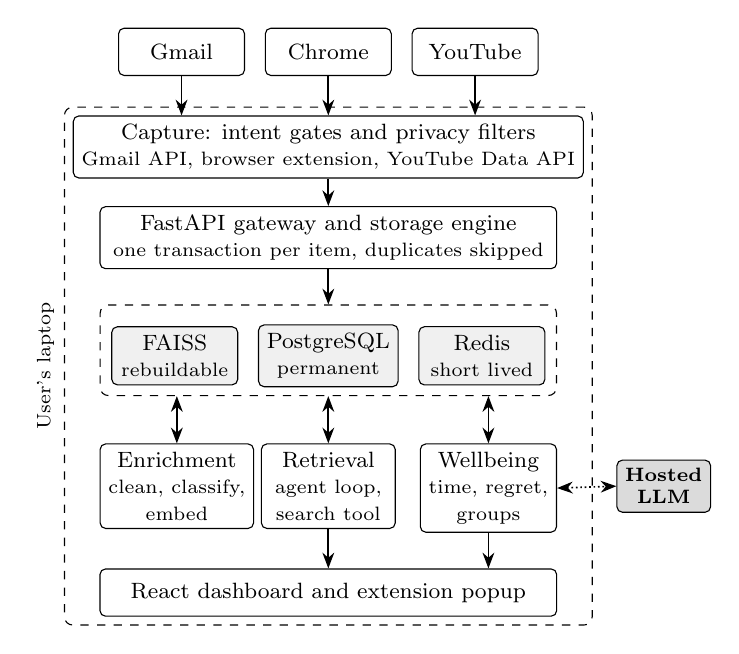
\begin{tikzpicture}[node distance=3.5mm and 2.5mm]
  \node[box, minimum width=16mm] (gm) {Gmail};
  \node[box, minimum width=16mm, right=of gm] (ch) {Chrome};
  \node[box, minimum width=16mm, right=of ch] (yt) {YouTube};
  \node[box, minimum width=58mm, below=5mm of ch] (cap)
      {Capture: intent gates and privacy filters\\ \scriptsize Gmail API, browser extension, YouTube Data API};
  \node[box, minimum width=58mm, below=of cap] (gw)
      {FastAPI gateway and storage engine\\ \scriptsize one transaction per item, duplicates skipped};
  \node[store, minimum width=16mm, below=7mm of gw] (pg) {PostgreSQL\\ \scriptsize permanent};
  \node[store, minimum width=16mm, left=of pg] (fa) {FAISS\\ \scriptsize rebuildable};
  \node[store, minimum width=16mm, right=of pg] (rd) {Redis\\ \scriptsize short lived};
  \node[grp, fit=(fa)(pg)(rd), inner ysep=5pt, yshift=2pt] (st) {};
  \node[box, minimum width=17mm, below=6mm of st.south west, anchor=north west] (enp)
      {Enrichment\\ \scriptsize clean, classify,\\ \scriptsize embed};
  \node[box, minimum width=17mm, below=6mm of st.south, anchor=north] (rse)
      {Retrieval\\ \scriptsize agent loop,\\ \scriptsize search tool};
  \node[box, minimum width=17mm, below=6mm of st.south east, anchor=north east] (wba)
      {Wellbeing\\ \scriptsize time, regret,\\ \scriptsize groups};
  \node[box, minimum width=58mm, below=5mm of rse] (ui) {React dashboard and extension popup};
  \node[grp, fit=(cap)(gw)(st)(enp)(wba)(ui), inner sep=3pt] (lap) {};
  \node[font=\scriptsize, rotate=90, anchor=south] at (lap.west) {User's laptop};
  \node[llm, minimum width=11mm, right=3mm of lap.east |- rse.east, anchor=west, font=\scriptsize\bfseries] (lm) {Hosted\\LLM};
  \draw[arr] (gm) -- (gm |- cap.north);
  \draw[arr] (ch) -- (cap);
  \draw[arr] (yt) -- (yt |- cap.north);
  \draw[arr] (cap) -- (gw);
  \draw[arr] (gw) -- (st.north);
  \draw[arr, {Stealth[length=2mm]}-{Stealth[length=2mm]}] (enp.north) -- (enp.north |- st.south);
  \draw[arr, {Stealth[length=2mm]}-{Stealth[length=2mm]}] (rse.north) -- (rse.north |- st.south);
  \draw[arr, {Stealth[length=2mm]}-{Stealth[length=2mm]}] (wba.north) -- (wba.north |- st.south);
  \draw[arr] (rse) -- (ui);
  \draw[arr] (wba.south) -- (wba.south |- ui.north);
  \draw[arr, densely dotted, {Stealth[length=2mm]}-{Stealth[length=2mm]}] (wba.east) -- (lm.west);
\end{tikzpicture}
\caption{The main parts of E.C.H.O. Everything inside the dashed frame runs on the user's laptop. The dotted arrow is the only path to the hosted language model of E.C.H.O; it carries bounded text from three callers (classification, retrieval, weekly reflection), described in Section~\ref{sec:privacy}.}
\label{fig:arch}
\end{figure}

% ---------------------------------------------------------------------
\section{Methodology}\label{sec:method}
% ---------------------------------------------------------------------
\subsection{Intent Aware Capture}
What should E.C.H.O keep? Each source has its own answer, and Table~\ref{tab:gates} summarizes them. These are the values we chose for the final system. The browser and the server hold matching copies, so that the server does not silently refuse a page that the extension sends.

Gmail is treated differently from the other two sources. Mail arrives on its own, so the user does not choose it. Also, few mails arrive each day, and even an unread message may matter later. So we store all messages when they arrive. The connector polls every 30 seconds, but each poll asks Gmail just for the changes since a saved history position. It does not list the entire mailbox each time. If that position has expired, the connector will list the mailbox once. Then the uniqueness rule on stored items absorbs the overlap. We do not read mail that Gmail has already filed as spam or trash, so Gmail's own spam filter also works as the spam filter of E.C.H.O. Whenever the user opens a message in Gmail on the web, the extension reports just the message id and the seconds spent reading.

For Chrome, the page is stored only if it passes the gate, and this gate has two phases. In phase one, the page has to stay in the foreground for at least five seconds. If a page fails this phase, we drop it, and we remember only a page that passes it for revisit detection. Phase two comes next, where at least one sign of attention has to appear. This sign can be enough foreground time, enough scrolling, a real interaction, or a visit to the same page within the last 24 hours. Selecting text or clicking inside the page counts as an interaction, but clicking a link does not. This is because a click that leaves the page shows a choice to go elsewhere, and not interest in the page itself. We count time only while the tab is active, the window has focus, and the user has not been idle for 30 seconds. Along with the text of the main content, the extension also sends the top level headings of the page, so that the page can be found later by its topic.

We keep a YouTube video if the user watches it long enough, or watches a large enough share of it. Pausing, seeking, changing the speed, or returning to the same video within a day also keeps it. The completion rule needs at least five seconds of real watching, such that swiping past a short clip does not count as watching ten percent of it. Once a video has been watched for five seconds, the extension records the visit, so that a second short visit can pass through the revisit rule. Shorts are recognized by their page address, and they get a lower time bar, 10 seconds instead of 20, as the clips themselves are short.

\begin{table}[t]
\caption{Capture Rules for Each Source}
\label{tab:gates}
\centering
\renewcommand{\arraystretch}{1.05}
\begin{tabular}{|>{\raggedright\arraybackslash}p{1.35cm}|>{\raggedright\arraybackslash}p{6.2cm}|}
\hline
\textbf{Source} & \textbf{An item is kept when} \\
\hline
Gmail & Always, at arrival, except mail in Spam or Trash. Polled every 30~s for changes only. Reading time is added when a message is opened (opens under 3~s are ignored). \\
\hline
Chrome & Phase 1: at least 5~s in the foreground. Phase 2: any one of at least 10~s in the foreground, at least 15\% scroll depth, one interaction other than a link click, or a revisit within 24~hours. Work app pages: at least 5~s or one interaction, title only. \\
\hline
YouTube & Any one of at least 20~s of foreground playback (10~s for Shorts), at least 10\% of the video watched with at least 5~s of watching, a pause, seek, or speed change by the user, or a revisit within 24~hours. \\
\hline
\end{tabular}
\end{table}

\subsection{Storage Model}
Each email, page, and video gets one row in a central \texttt{memory\_items} table. What is specific to Gmail, Chrome, or YouTube goes into a matching source table, and attachments have their own table. Engagement counters such as reading time, watch time, and revisits change often, so they are kept apart from the item. Suppose a page is read on Monday and then again on Thursday, it should count on both days, but with only one ``last seen'' time, Thursday simply replaces Monday. That is why \texttt{visits} exists, every admitted visit from Chrome or YouTube gets its own row in it, when the visit happened and how many seconds were spent. The schema has 17 tables in total.

The same item can come in twice, mainly when a connector restarts or when the Gmail connector has to list the mailbox again, and we don't want to store it twice, so there is a uniqueness rule on source type and source id together. When a new item comes it is written raw first, with an unprocessed flag on it. Enrichment we kept separate on purpose, because it takes a few seconds for every item and capture can't wait for that, and even if the worker crashes, capture should keep running. Every item also gets one of the 5 system groups, misc being the fallback. Then if a page is revisited and the text has changed, it is flagged again and the vector gets rebuilt. Timestamps we store in UTC and show in local time.

Once the user deletes an item, no query can see it anymore. Retention is forever by default, the whole point is recalling something like a mail from last year, but one year or six months can also be picked. With a shorter window a job at backend startup removes the old items from PostgreSQL, FAISS and Redis together, together because if an item is gone from PostgreSQL but still in FAISS it can come back as a search hit.

\subsection{Background Enrichment}
A background worker picks up the unprocessed items every few seconds. The worker is outside the capture path. So if some step is slow it only delays when the item becomes searchable, capture will not wait for it. There are four steps for each item, and the last thing that happens is recording its final state.

\textit{Cleaning.} For email, HTML is converted to text with the line breaks kept, and scripts, styles, tracking pixels, and hidden preview text are removed. When the sending app has split a body around an inline image, the parts are joined back together. Quoted earlier messages are removed, but the lines the sender typed between quoted lines are kept. This is because an inline reply is often the most important part of the message. A heuristic remover that we tested cut real body text in six of eight sample messages, while a leftover signature only adds a little noise. So signatures are deliberately left in place, as a little noise is better than lost body text. For a reply, keywords from earlier messages in the same thread are added, so that a terse ``Re:'' can still be found by its topic. For web pages, the extension has already picked the main content and the headings, and the worker separates the headings from the body. A video's text is made of its title, channel, category, tags, and description. The server also tries to download the caption text, but this is best effort, and it returned nothing for any of the 14 videos in our test data.

\textit{Attachments.} The same worker extracts attachment text when the mail is processed. It supports PDF, DOCX, XLSX, PPTX, HTML, forwarded messages, and plain text formats such as TXT, CSV, Markdown, JSON, and calendar files. Images and scanned PDFs are read with Tesseract OCR \cite{b15}, while inline images such as signature logos, and very small images, are skipped. The extracted text is stored next to the attachment record and not inside the email body. The beginning of each attachment joins the embedded text of the email, while the entire text joins the keyword index. So a line deep inside a file, say a clause in an offer letter or a date in a flight itinerary, can still be found by keyword. Both kinds of file are among the five PDFs in our test data.

\textit{Embedding.} We embed with the \embmodel{} sentence model \cite{b16}, which replaced \texttt{all-\allowbreak MiniLM-\allowbreak L6-\allowbreak v2} in our system. It reads at most 512 tokens and produces a 384 dimension vector. Since the window is fixed, the order of the text decides what gets lost when an item is too long. Short hints go first, for mail that is the subject, keywords and sender, for pages the domain and headings, and for videos the channel and category. The long text, like the email body or the description, goes last, because if something has to be cut, it should be the end of a long body and not what people remember. Now the model's own tokenizer makes the cut, it stops at a whole word, and what we store and what got embedded is the same text exactly. When a mail has attachments, up to 300 tokens go to the body and whatever is left goes to the attachments. For a video the description gets up to 200 tokens, the captions fill the rest. Then the vector is added to FAISS without a rebuild.

\textit{Classification.} Every item gets one of five broad groups, work, study, entertainment, personal and misc, the offer letter in our data for example went into personal, and misc is for anything that fits nowhere. A cascade of four stages picks the group, and an item moves on to the next stage only if the current one cannot place it. Stage one is the structural signals from the source, a Gmail label like Promotions, an academic mail domain, the YouTube category, and stage two looks the web domain up in a curated table so a known site gets its group without any model. The cheap stages do most of the work, that was the idea, and on the 119 test items it held. Structural signals placed 84 items (70.6\%), the domain table 5 (4.2\%), and the group centers of stage three 11 (9.2\%). Only 19 (16.0\%) went to the language model.

Stage three compares the item's vector with a center for each group and accepts only a clear winner. A center starts as a seed, the mean of several example sentences written for its group. A seed has to lead the second best group by at least 0.05, a value we measured on labeled rows (Section~\ref{sec:eval}). After a group has ten confirmed items, its center is recomputed from them, with all sources weighted equally, so the center learns the topic instead of the look of one source. Both kinds of center need a cosine similarity of at least 0.55, and a recomputed one also has to be ahead by 0.08 or more. At worker startup the centers get recomputed, that is if they are missing or more than 30 days old. In stage four the language model gets one item at a time, the title and about 300 characters. With OpenAI it is a typed choice among the 5 group names, with other providers the reply has to be exactly one group name, and if it is anything else it becomes misc. Classification doesn't stop even when the typed call fails, the item just falls back to the single word path. We do not store a confidence value.

\textit{State tracking.} Each item ends up processed or failed. Failed ones are set aside. They are not counted as done and not lost, a configuration switch lets the worker retry them.

\subsection{Retrieval Loop}
A question goes through the loop shown in Fig.~\ref{fig:graph}. The model, \llmname{}, receives the conversation so far, the question, one tool called \texttt{search\_memories}, and a small calendar around today's date, which takes the place of a separate date parser. The main argument of the tool is a query of a few keywords, and it comes with some options. These are up to two alternative phrasings, a list of sources, a start date, a reference item with the word before or after, and a flag to ask for attachment text. The model decides how to phrase the search. Then, in one round, it may issue several searches in parallel, for instance one per source. After reading the results, it either answers directly or searches again. On the first turn of a chat, the first call has to use the tool. A usual question needs one call that searches and one call that answers. The code allows at most five searches for one question, and at most three in one round. After the fifth search, we make the next call without the tool, such that the model has to answer. So a question costs between two and six model calls, and the program enforces this bound, not the prompt.

\begin{figure}[t]
\centering
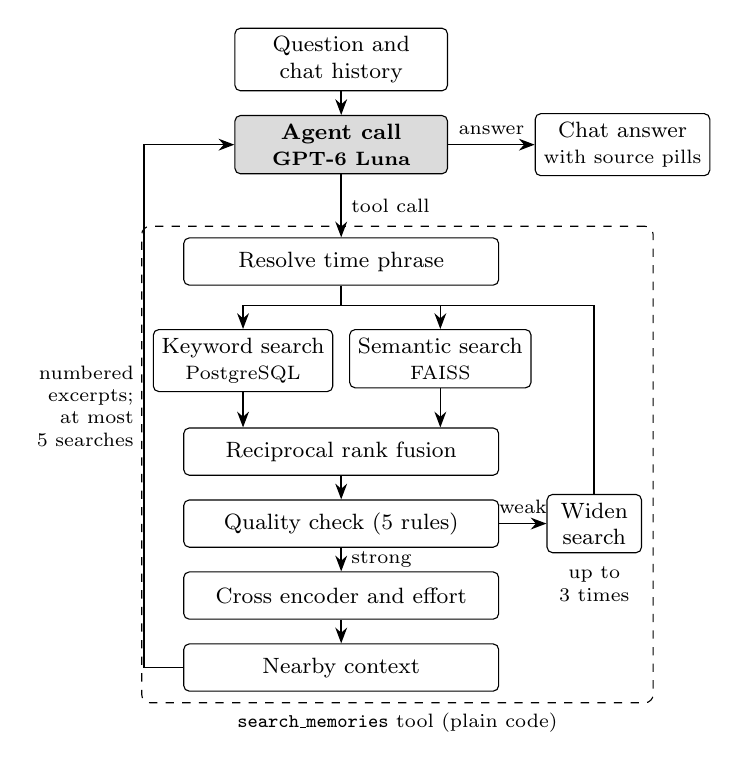
\begin{tikzpicture}[node distance=3mm and 3mm]
  \node[box, minimum width=27mm] (q) {Question and\\ chat history};
  \node[llm, minimum width=27mm, below=of q] (ag) {Agent call\\ \scriptsize\llmname};
  \node[box, minimum width=22mm, right=11mm of ag] (an) {Chat answer\\ \scriptsize with source pills};
  \node[box, minimum width=40mm, below=8mm of ag] (ta) {Resolve time phrase};
  \coordinate (bus) at ($(ta.south)+(0,-2.5mm)$);
  \node[box, minimum width=19mm, anchor=north east] (kw) at ($(bus)+(-1mm,-3mm)$) {Keyword search\\ \scriptsize PostgreSQL};
  \node[box, minimum width=19mm, anchor=north west] (se) at ($(bus)+(1mm,-3mm)$) {Semantic search\\ \scriptsize FAISS};
  \node[box, minimum width=40mm, anchor=north] (rrf) at ($(bus)+(0,-15.5mm)$) {Reciprocal rank fusion};
  \node[box, minimum width=40mm, below=of rrf] (qc) {Quality check (5 rules)};
  \node[box, minimum width=12mm, right=6mm of qc] (wd) {Widen\\search};
  \node[box, minimum width=40mm, below=of qc] (ce) {Cross encoder and effort};
  \node[box, minimum width=40mm, below=of ce] (nb) {Nearby context};
  \node[grp, fit=(ta)(kw)(se)(rrf)(qc)(wd)(ce)(nb), inner sep=4pt] (tool) {};
  \node[font=\scriptsize, anchor=north] at (tool.south) {\texttt{search\_memories} tool (plain code)};
  \draw[arr] (q) -- (ag);
  \draw[arr] (ag) -- node[above, font=\scriptsize] {answer} (an);
  \draw[arr] (ag) -- node[right, font=\scriptsize] {tool call} (ta);
  \draw[semithick] (ta.south) -- (bus);
  \draw[semithick] (bus -| kw.center) -- (bus -| wd.center);
  \draw[arr] (bus -| kw.center) -- (kw.north);
  \draw[arr] (bus -| se.center) -- (se.north);
  \draw[semithick] (wd.north) -- (wd.north |- bus);
  \node[font=\scriptsize, align=center, below=0.5mm of wd] {up to\\3 times};
  \draw[arr] (kw.south) -- (kw.south |- rrf.north);
  \draw[arr] (se.south) -- (se.south |- rrf.north);
  \draw[arr] (rrf) -- (qc);
  \draw[arr] (qc) -- node[above, font=\scriptsize] {weak} (wd);
  \draw[arr] (qc) -- node[right, font=\scriptsize] {strong} (ce);
  \draw[arr] (ce) -- (nb);
  \draw[arr] (nb.west) -- ++(-5mm,0) |- node[pos=0.25, left, font=\scriptsize, align=right] {numbered\\excerpts;\\at most\\5 searches} (ag.west);
\end{tikzpicture}
\caption{The retrieval loop. A language model gets called only in the shaded box. Everything inside the dashed frame is deterministic code, along with two small local encoders. When the search is widened, both search branches run again.}
\label{fig:graph}
\end{figure}

\textit{Resolve time phrase.} The model reads the calendar in its first message and passes a start date, so a phrase such as ``last Tuesday'' reaches the tool as a date. The tool accepts only a valid date. A phrase that points at another item, such as ``after the interview email,'' is passed as a reference item, and the code looks it up among the user's own items. The lookup tries keywords first and meaning second, with a minimum similarity. Once it finds the item, that item's time becomes a hard limit for both search branches. If no reference item is found, the search runs without that limit. An email counts as inside the range by its arrival time. A page or a video counts if any one of its recorded visits does. The date filter is open ended, so the answering call is told today's date and asked to use only the items inside the period the user named. Section~\ref{sec:eval} shows how our own test question of this kind, ``after the Brightwave interview email,'' turned out.

\textit{Parallel search.} Two branches search at once, in the same step of the graph. The semantic branch embeds the query and looks it up in FAISS. Titles, full item text, attachment text, senders, domains and channel names, all of these go into one stored column, \texttt{search\_vector}, with a GIN index on it, and the keyword branch runs PostgreSQL full text search over that column. That is why a question like mail from one person works, the name of that person is right there to match on.

\textit{Fusion.} The two ranked lists are merged with reciprocal rank fusion \cite{b9}. For an item $d$, the fused score is
\begin{equation}
\mathrm{RRF}(d) = \sum_{b \in B} \frac{1}{k + r_b(d)}, \label{eq:rrf}
\end{equation}
where $B$ is the set of branches that returned $d$, $r_b(d)$ is its position in branch $b$ starting from 1, and $k = 60$. PostgreSQL text rank and cosine similarity are on different scales, a good match for us was around 0.7 in cosine while text rank is on its own scale, so adding them would not mean anything and positions are used instead. The top 50 fused items move on to the next step.

\textit{Quality check and widening.} Five rules judge the fused list. We call a list weak in four cases, it is empty or has under 2 items, nothing in it is from a source the user wanted, nothing falls in the time window, or its top cosine similarity is under 0.55. The 0.55, it sits in a narrow gap, the weakest answerable query was 0.558 and the best unanswerable was 0.573, so at 0.55 none of the 38 answerable queries got flagged and 2 of the 12 unanswerable got through (Section~\ref{sec:eval}). Then both branches run again, this time on a wider search. First widening adds 4 days to the time window, opens all sources or cuts the query to its core keyword. The second drops the time filter and the anchor. The third drops the keyword filters and searches a larger part of the vector index. If all three fail, the tool reports that nothing was found, and the model can then tell the user so or try another phrasing.

\textit{Reranking.} The local cross encoder \rerankmodel{} \cite{b10}, \cite{b11} scores each remaining item against the question. It reads the title of the item followed by the beginning of its cleaned text, 512 characters in all. The final score blends this with an effort score:
\begin{equation}
s(d) = 0.8\,\sigma\big(c(q,d)\big) + 0.2\,e(d), \label{eq:final}
\end{equation}
where $c(q,d)$ is the cross encoder output for question $q$ and item $d$, $\sigma$ is the sigmoid function, and $e(d) \in [0,1]$ is the effort score. Effort is the mean of the engagement signals that an item has, such as reading or watch time, scroll depth, revisits, interactions, and how much of a video was watched. Each signal is capped and scaled to $[0,1]$. This favors the items that the user gave real attention to. Email is a special case. If a mail was read on a phone, or never opened in the browser, it has no measurable reading time. Instead of scoring such mail as zero, the reranker gives it the median effort of the other emails in the same result list. This way, an unmeasured email is neither punished nor promoted. By design, the score has no term for how recent an item is, and there is no diversity reranking.

\textit{Nearby context and excerpts.} The top three items bring their close neighbors with them, meaning other emails in the same thread, or pages and videos from the same browsing session or within five minutes. The model sees each result as a numbered entry. The top 3 entries get 8,000 characters of the cleaned text and the rest get 2,000, and along with that opening text each entry carries the title, source, time, and the sender, site or channel. Questions about an attachment get one more thing, up to 40,000 characters of extracted text from the attachment of the best ranked mail. That is a lot of room actually, even the biggest request we sent in the evaluation came to 38,469 characters (Section~\ref{sec:eval}). And one question can need several searches, but the numbering of entries doesn't change between them, so whatever a citation points to, it is that same item every time.

\textit{Writing the answer.} The last call is the one that writes the reply, in Markdown, more like a conversation. Direct answer first. If something is not there, it just says it is missing, and if the question is ambiguous it asks back, one line. Now each fact has a hidden marker with it, naming which numbered item it came from, and the backend checks these markers and keeps only the ones pointing to items that the tool actually returned, so the model can't cite something it never saw. On the screen these markers show up as small pills, sender or site or channel with a short date. We did it this way because when we think of an email, we remember who sent it and roughly when. Click a pill and the original opens. Below the reply there is also a thin time strip that puts the cited items on a timeline. While the loop is running, the dashboard shows progress messages, such as which source it is searching.

\textit{Failure handling.} If the model cannot be reached, the deterministic pipeline runs once on the raw question. In this case, the user still receives the ranked list of matching items, and not an error.

\subsection{Conversation Memory}
Each chat has a session id, and we save every turn in PostgreSQL on the laptop. When the user opens an old chat, its session picks up from where it was left. So a follow up such as ``show me Chrome pages about that topic after that email'' can refer back to an earlier answer. A new turn sends the model the last twelve messages, with each question cut to 1,000 characters and each answer to 3,000, so that a long old answer cannot take over the context meant for the new question. The citation numbers restart with every question. When the backend comes up, chats which are older than 30 days are removed, so the history goes back about a month only.

% ---------------------------------------------------------------------
\section{Wellbeing and User Groups}\label{sec:wba}
% ---------------------------------------------------------------------
The wellbeing module is built around one question: where did my time go? We gave the module one rule. It shows numbers and patterns, it gives the user no score, and nothing in it calls time wasted. Whether that time was well spent or not, that is the user's call.

\textit{Time.} We never store a time total. Whenever one is needed it is worked out from the records, that way no minute gets counted twice. Page and video time comes from \texttt{visits} (Section~\ref{sec:method}), so each day gets exactly its own time. Email time is from the reading time the extension reports, and the days are the user's local days.

\textit{Sessions.} Consecutive items which are under 20 minutes apart, that is one session for us. At first we planned 5 minutes but it was splitting one sitting into two, so we moved it to 20, because each item is only one point in time, if someone reads a page for 15 minutes and then opens the next one the record shows a 15 minute gap, but the user never left. For each session we keep the length, the system group with most time, and how many times the user switched between sources.

\textit{Regret.} Any item can be marked, and what counts as regret is for the user alone to decide. Each mark or unmark goes in as a new event and not as a yes or no field, people change their mind and we wanted that history kept, and an item is regretted right now when its event count is odd. The module reports marked items per content type and per hour, and if the same kind of item, say a YouTube Short, is marked at a similar hour at least 3 times in 30 days, it is flagged as a habit.

\textit{Weekly reflection.} Once a week, the module can write a short reflection. For this, one language model call receives only aggregated numbers, which are totals per category, regret counts, session patterns, and peak hours. It does not receive a title, an address, or any text from an item. Before the reply is shown, it is checked for judging phrases. If it fails this check, or if the call itself fails, a simple summary built from the same numbers is shown instead.

\textit{User groups.} System groups answer ``what kind of item is this?'', while user groups answer ``which of my goals does it serve?'', for example ``Placement prep.'' A user group starts with the items that the user files by hand. Once it has five confirmed items, an assignment job scores other items against it in two ways. The first way uses the rules the user wrote, each on a keyword, domain, channel, sender, or date range. The second way is a nearest neighbor score, which is the mean cosine similarity between the item and the three most similar confirmed members. An item is suggested when a rule matches, or when the neighbor score alone reaches a threshold. We set this threshold to 0.85, the lowest value at which no item outside a group scored at or above it in our test (Section~\ref{sec:eval}). The module can also propose a new rule when at least five confirmed members share a domain, sender, or channel.

When does E.C.H.O add something on its own? It does so only for a confident suggestion. A suggestion is confident if a rule matches and the neighbor score also reaches that same threshold. We add such an item directly, but the item still appears in the weekly review, where one click undoes it. So we handle confident items with a human on the loop. Anything less certain waits for an explicit accept in the review screen, which means the human stays in the loop. Also, an automatic addition does not count as a confirmed member until the user keeps it. So one wrong addition cannot pull in the next similar item. Manual filing and automatic additions pass through the same recorded path, so each membership has an audit trail. We never offer a rejected or removed suggestion again for that group. User groups are independent of the five system groups and have no parent among them, such that one goal can hold study pages and work mail together.

% ---------------------------------------------------------------------
\section{Privacy by Design}\label{sec:privacy}
% ---------------------------------------------------------------------
\textit{What is never captured.} Nothing from incognito windows is recorded, and the same goes for typed text and form input. Some pages also keep no text at all. A page falls in this case when its address contains a sensitive word, such as login, password, checkout, otp, or netbanking. Each word is matched as a whole word against a fixed list of 38. A page with a visible password box, or with a form of several personal fields, is treated the same way. Parameters that often carry secrets, such as tokens, one time codes, and session ids, are cut from every address before it is stored. Seven work apps, which are Slack, Atlassian, Notion, Figma, Linear, Trello, and Asana, are stored only as page titles and not as text. Their public help, blog, and documentation sections are still treated as ordinary pages. Gmail on the web is skipped by browser capture, because the mail already arrives through the Gmail API. All these lists live in one copy on the server, and the extension fetches them at startup. Until they arrive, the extension extracts no text.

\textit{What leaves the laptop.} The database, the vector index, the cache, and both encoders run locally. Two kinds of traffic leave the machine. First, requests to the Gmail and YouTube APIs fetch the user's own data. Second, calls to the hosted language model carry text from three callers. Retrieval sends the question, the recent chat history, and the numbered results. Each result is a title, a time, a sender, site, or channel, and the beginning of its text, at most 8,000 characters for each of the top three results and 2,000 for the others. When the user asks about a file, the text of one attachment is added, at most 40,000 characters. The classifier sends a title and about 300 characters, and it does so only for the items that the first three stages could not place. The weekly reflection sends only aggregated numbers. So a short email can reach the model whole, but a longer email, a page, or a transcript never does beyond these limits, and database rows and vectors are never sent. Requests to the hosted service are also subject to the data retention policy of its provider. Also, when the user connects an MCP client (Section~\ref{sec:impl}), the tool results go to that client, so its own language model sees the same excerpts.

\textit{Captured text is treated as data.} A newsletter or a web page can contain text written for a language model, such as ``ignore your previous instructions.'' This is known as prompt injection. In E.C.H.O, the worst such text can do is shape a search or an answer. It cannot delete or send anything, the only tool the model has is read only. And in the system prompt we tell the model, whatever comes back from the tool is the user's data, it is not instructions. Even the retrieval logs we kept small, counts, scores and timings, the question and the title are never logged.

\textit{User control.} Each source can be turned on or off from the Settings page, and that is also where the user picks how long data is kept. To stop for a while there is a switch in the extension popup that pauses capture. Domains and senders can be excluded, for example a bank site or one sender, single items deleted, all data exported as JSON or CSV, and if retention is shorter than forever the old data is removed permanently.

% ---------------------------------------------------------------------
\section{Implementation}\label{sec:impl}
% ---------------------------------------------------------------------
Table~\ref{tab:stack} has the full stack. We wrote the backend in Python and it is served with FastAPI, the retrieval loop is a LangGraph graph \cite{b5} where an agent node and a tool node take turns under a round counter. Every model call goes through LangChain so changing the provider is one config entry, \texttt{LLM\_CONFIG} in \texttt{rse/config.py}, and this we actually did when we moved from Gemini to OpenAI, we only edited that entry. If the provider is OpenAI, the code also turns on the features that are specific to it. Those features are the Responses API, medium reasoning effort on both of the retrieval calls and the typed choice for the classifier. The embeddings and the cross encoder run locally on the CPU through the sentence transformers library. We built the dashboard with React and TypeScript, and the extension uses Chrome Manifest V3.

PostgreSQL 16 runs as a native service on the laptop, and Redis runs locally under the Windows Subsystem for Linux. So both stay on the laptop, and only standard HTTPS traffic leaves the machine.

E.C.H.O also runs as a server for the Model Context Protocol (MCP) \cite{b17}. Over the stdio transport, it exposes two read only tools, \texttt{search\_memories} and \texttt{get\_memory}. The first one has the same contract as the tool in the retrieval loop. So any MCP client, such as Claude Desktop, can query the memory with its own language model. In that case, the client plans the searches instead of the agent loop, while E.C.H.O stays the engine that does the actual searching.

\begin{table}[t]
\caption{Technology Used in the Final System}
\label{tab:stack}
\centering
\renewcommand{\arraystretch}{1.05}
\begin{tabular}{|>{\raggedright\arraybackslash}p{1.6cm}|>{\raggedright\arraybackslash}p{5.95cm}|}
\hline
\textbf{Layer} & \textbf{Technology} \\
\hline
Capture & Chrome extension (Manifest V3), Gmail API, YouTube Data API \\
\hline
Backend & Python, FastAPI, server sent events \\
\hline
Storage & PostgreSQL 16, FAISS, Redis, all local \\
\hline
Enrichment & Text extraction for PDF, DOCX, XLSX, PPTX, and EML; Tesseract OCR \\
\hline
Models & \embmodel{} embeddings (\embdim{} dimensions, 512 tokens),\newline \rerankmodel{} cross encoder,\newline \llmname{} through the OpenAI Responses API \\
\hline
Retrieval & LangGraph, LangChain, MCP Python SDK (stdio) \\
\hline
Interface & React, TypeScript, Vite \\
\hline
\end{tabular}
\end{table}

% ---------------------------------------------------------------------
\section{Evaluation}\label{sec:eval}
% ---------------------------------------------------------------------
\subsection{Setup}
We evaluated E.C.H.O on just one test account, which belongs to the authors. It holds 119 items, which are 78 emails, 30 pages, and 11 videos. Five of the emails carry a PDF attachment, and we extracted its text. We prepared 38 questions of five kinds. There are 16 about one item in one source, 4 about several sources, 6 with a time reference (``emails I received today,'' ``after the interview email''), 6 follow up questions that refer to an earlier turn, and 6 about the content of an attachment. Before the run, the relevant items for each question were marked. There are 81 of them in all, with at most eight for one question. We ran everything on one Windows laptop and called the hosted model through its API.

\subsection{Retrieval Quality}
We compare five configurations. The first four replay, for each question, the arguments that the model chose in its first search, so that they differ only in the stages of the tool. These are keyword search alone, semantic search alone, fusion without the cross encoder, and the full pipeline with quality check, widening, and reranking. The fifth is the whole agent loop. Table~\ref{tab:results} gives Recall@10, Recall@5, and the mean reciprocal rank (MRR) of the first relevant item within the first ten results. Recall@$k$ counts the relevant items among the first $k$ results and divides that by the smaller of $k$ and the number of relevant items.

\begin{table}[t]
\caption{Retrieval Quality on 38 Questions}
\label{tab:results}
\centering
\renewcommand{\arraystretch}{1.05}
\begin{tabular}{|l|c|c|c|}
\hline
\textbf{Configuration} & \textbf{R@10} & \textbf{R@5} & \textbf{MRR} \\
\hline
Keyword only & 0.697 & 0.697 & 0.693 \\
\hline
Semantic only & 0.955 & 0.934 & 0.987 \\
\hline
Fusion, no cross encoder & 0.955 & 0.934 & 0.987 \\
\hline
Full pipeline & 0.927 & 0.905 & 0.899 \\
\hline
Full agent loop & 0.927 & 0.905 & 0.899 \\
\hline
\end{tabular}
\end{table}

Keyword search alone reaches a recall of 0.70, because the full text search needs every query word to match, and for 11 of the 38 questions it found no relevant item. Semantic search alone and its fusion with keyword search both reach 0.955 with an MRR of 0.987. So on this collection, the keyword branch did not change the first ten results. Now the full pipeline scores lower. For five questions, the right item moved from first place to second or third place after reranking. In the two questions that we examined in detail, the cross encoder gave scores below 0.01 to all candidates. So the effort term of Eq.~\eqref{eq:final} decided the order, and an email that the user had opened outranked the right one. We therefore cannot claim that reranking helps on small collections of this kind.

The agent loop and the full pipeline have the same top ten, because later searches add items after the first ten. The loop pays off when we count everything it showed to the model. That was 70 of the 81 relevant items, against 65 for a single pass (0.86 against 0.80), at the cost of showing more results. The gain came from three questions in which a second search found items that the first one missed. By kind of question, the loop recall was 1.00 for single source, follow up and attachment questions, but 0.74 for several sources and 0.71 for a time reference. Part of the time loss is the open date filter, a question with only a start date has no end, so later items crowd in. In the question ``after the Brightwave interview email,'' the model wrote the phrase into the query and did not use the reference item, which gave a recall of 0.20. The answers to all 11 questions whose answer contains a unique fact were correct.

\subsection{Cost and Speed}
The 38 questions made 44 turns, since each follow up has two. A turn needed 2.34 model calls on average. In detail, 33 turns used two calls, 8 used three, 2 used four, and 1 used five. No turn used all five searches, the budget never got fully used. Four was the most. The median response time was 8.1 seconds, the 95th percentile was 23.8 seconds, and the longest was 30.2 seconds. On average, a turn sent 8,983 input tokens and received 238 output tokens. At an assumed price of 0.20 and 1.20 US dollars per million input and output tokens, this comes to about 0.002 dollars per turn.

\subsection{Capture Accuracy}
We replayed 15 scripted browsing and viewing sessions in a test profile of Chrome with the extension. The sessions include a page closed after three seconds, a page read for six seconds without scrolling, a page scrolled to 20 percent, a click on a link, and a text selection. They also include a page address with a secret parameter, a video closed after three seconds, a ten minute video watched for seven seconds twice, and a video watched for 25 seconds. Before the run, we wrote down the expected result of each session from the rules. Thirteen sessions were clean, and in all 13 the stored items matched the rules (8 Chrome and 5 YouTube sessions). Two further sessions were discarded because a person used the browser during them. A script drove the sessions and also kept the system from going idle, and the durations are accurate to about two seconds.

\subsection{Privacy Audit}
During the evaluation, we recorded all requests to the language model. The largest request held 38,469 characters. Two items in the collection are longer than the 8,000 character limit for the top results, and both were shown to the model. The text beyond the limit appeared in no request.

\subsection{Threshold Calibration}
Three similarity cutoffs depend on the embedding model, so we measured them on the collection. First, we looked at the seed centers of classification stage three. For this we used 78 items, ones where the structural signals already told us the group. A lead of 0.08 didn't fire even once on these, 0.05 fired 14 times and all 14 were correct, and no item was below 0.585, so the 0.55 floor, that never got tested.

For the quality check, the 38 answerable queries never went below 0.558 for the best similarity, the median was 0.734, and the 12 unanswerable ones went at most 0.573. So 0.55 doesn't flag any good query, but 2 of the 12 bad ones get through. We thought of 0.58, which would stop those 2, but then 1 good one gets flagged wrongly, and one query is not really evidence, so we stayed with 0.55.

Then the user groups. Three groups, 13, 5, and 5 items. Every member got scored against the others in its own group, and each group was also scored against all the other items. At 0.65 all 23 members pass, but 155 of the 358 other items also pass, which is too many. At 0.85 only 7 members pass and nothing else, so 0.85 is the lowest value without a wrong item, and that's what we use, even though on meaning alone only about 30\% of the real members reach it. So most suggestions will come from the user's rules and not from similarity. All of this is on a small sample, with groups and labels that are still provisional.

% ---------------------------------------------------------------------
\section{Limitations and Future Work}\label{sec:limits}
% ---------------------------------------------------------------------
Coverage, that is the biggest limit. E.C.H.O sees only desktop Chrome, so anything done on a phone is missing. Anything watched before the extension was installed is not in the YouTube history, and background playback or picture in picture is not tracked either. One vector per item means only the first 512 tokens shape the meaning match, anything deeper we can reach only through keyword. Then with Outlook, a reply carries the older thread inside it and there is no marker for E.C.H.O to strip it by, so one thread can appear more than once. The date filter is open ended, and only the top ten results of each search reach the answering call. So if today was busy, today's items can crowd out what a question about yesterday should find. Classification has a weak spot too, stage one trusts the Gmail labels, Gmail had marked an offer letter and a course syllabus as Personal, so E.C.H.O also marked them as personal. Private apps outside the seven listed, chat assistants or online documents for example, get captured as normal pages unless the domain is excluded. OAuth tokens are plain files, with only the OS file permissions protecting them. Captions are best effort, for our videos none came back, so a video's text is title, tags and description only.

Some things we could not test at all, scanned files for one, because Tesseract was not installed in the test setup, and the wellbeing module and group suggestions were never tried with users. What we did test is one account with 119 items and 38 questions, prepared within the project and not by independent users, so one question is about 2.6 percentage points of recall, and with bigger collections or other users it may not hold. With ``after the Brightwave interview email,'' the reference item never got passed, the model wrote that phrase into the query instead, and some relevant items were lost. And we depend on a hosted language model, so whatever its availability and limits are, they apply to us too.

Reranking is first, because that is where the results hurt the most, the engagement weight outweighed relevance and MRR fell from 0.987 to 0.899, which means the right item was getting pushed from first place to second or third. After that comes a bigger evaluation, with several users, and questions from people who did not build the system. We also want several vectors per long item, a domain table that learns from labels the user confirms, and importing past history from Google Takeout and the browser's history file so a new user does not start empty.

% ---------------------------------------------------------------------
\section{Conclusion}\label{sec:conc}
% ---------------------------------------------------------------------
So E.C.H.O is one memory over a person's email, browsing and video history, and they can ask it questions. All legitimate mail it keeps, but only the pages and videos that got attention, everything is on the laptop and gets prepared in the background. The planning is done by the model and the searching by plain code, so the model's role stays visible, its calls are bounded and the cost is low. As for the wellbeing module, it describes time and the personal groups stay in the user's charge. On 119 items a question took 2.3 model calls and a median of 8.1 seconds, and 93\% of relevant items were in the first ten. Most of what we learned came from the parts that did not work. Most of the ranking on a small personal collection got done by a good small embedding model and the cross encoder added nothing on top, and the model also did not always use the reference to another item. The one place the loop did help was recall, over several searches the model got to see 0.86 of the relevant items, while a single pass showed only 0.80.

\section*{Acknowledgment}
We are thankful to the Department of Computer Science and Engineering, PES University for supporting this capstone. The faculty who reviewed our work in every phase, we also thank them, for all the questions they asked and the feedback they gave.

\IEEEtriggeratref{99}
\begin{thebibliography}{00}
\bibitem{b1} V. Bush, ``As we may think,'' \textit{The Atlantic Monthly}, vol. 176, no. 1, pp. 101--108, Jul. 1945.
\bibitem{b2} S. Dumais, E. Cutrell, J. J. Cadiz, G. Jancke, R. Sarin, and D. C. Robbins, ``Stuff I've seen: A system for personal information retrieval and re-use,'' in \textit{Proc. 26th Annu. Int. ACM SIGIR Conf. Research and Development in Information Retrieval}, Toronto, Canada, 2003, pp. 72--79.
\bibitem{b3} J. Gemmell, G. Bell, and R. Lueder, ``MyLifeBits: A personal database for everything,'' \textit{Commun. ACM}, vol. 49, no. 1, pp. 88--95, Jan. 2006.
\bibitem{b4} P. Lewis, E. Perez, A. Piktus, F. Petroni, V. Karpukhin, N. Goyal, H. K\"{u}ttler, M. Lewis, W. Yih, T. Rockt\"{a}schel, S. Riedel, and D. Kiela, ``Retrieval-augmented generation for knowledge-intensive NLP tasks,'' in \textit{Advances in Neural Information Processing Systems}, vol. 33, 2020, pp. 9459--9474.
\bibitem{b5} LangChain, ``LangGraph,'' GitHub repository. [Online]. Available: \url{https://github.com/langchain-ai/langgraph} (accessed Oct. 21, 2026).
\bibitem{b13} S. Yao, J. Zhao, D. Yu, N. Du, I. Shafran, K. Narasimhan, and Y. Cao, ``ReAct: Synergizing reasoning and acting in language models,'' in \textit{Proc. 11th Int. Conf. Learning Representations (ICLR)}, Kigali, Rwanda, 2023.
\bibitem{b6} N. Reimers and I. Gurevych, ``Sentence-BERT: Sentence embeddings using Siamese BERT-networks,'' in \textit{Proc. 2019 Conf. Empirical Methods in Natural Language Processing and 9th Int. Joint Conf. Natural Language Processing (EMNLP-IJCNLP)}, Hong Kong, China, 2019, pp. 3982--3992.
\bibitem{b16} L. Merrick, D. Xu, G. Nuti, and D. Campos, ``Arctic-Embed: Scalable, efficient, and accurate text embedding models,'' arXiv:2405.05374, 2024.
\bibitem{b8} J. Johnson, M. Douze, and H. J\'{e}gou, ``Billion-scale similarity search with GPUs,'' \textit{IEEE Trans. Big Data}, vol. 7, no. 3, pp. 535--547, Jul. 2021.
\bibitem{b9} G. V. Cormack, C. L. A. Clarke, and S. B\"{u}ttcher, ``Reciprocal rank fusion outperforms Condorcet and individual rank learning methods,'' in \textit{Proc. 32nd Int. ACM SIGIR Conf. Research and Development in Information Retrieval}, Boston, MA, USA, 2009, pp. 758--759.
\bibitem{b10} R. Nogueira and K. Cho, ``Passage re-ranking with BERT,'' arXiv:1901.04085, 2019.
\bibitem{b7} W. Wang, F. Wei, L. Dong, H. Bao, N. Yang, and M. Zhou, ``MiniLM: Deep self-attention distillation for task-agnostic compression of pre-trained transformers,'' in \textit{Advances in Neural Information Processing Systems}, vol. 33, 2020, pp. 5776--5788.
\bibitem{b11} P. Bajaj \textit{et al.}, ``MS MARCO: A human generated machine reading comprehension dataset,'' arXiv:1611.09268, 2016.
\bibitem{b12} M. Kleppmann, A. Wiggins, P. van Hardenberg, and M. McGranaghan, ``Local-first software: You own your data, in spite of the cloud,'' in \textit{Proc. ACM SIGPLAN Int. Symp. New Ideas, New Paradigms, and Reflections on Programming and Software (Onward!)}, 2019, pp. 154--178.
\bibitem{b14} U. Lyngs \textit{et al.}, ``Self-control in cyberspace: Applying dual systems theory to a review of digital self-control tools,'' in \textit{Proc. CHI Conf. Human Factors in Computing Systems (CHI '19)}, Glasgow, UK, 2019, doi: 10.1145/3290605.3300361.
\bibitem{b15} R. Smith, ``An overview of the Tesseract OCR engine,'' in \textit{Proc. 9th Int. Conf. Document Analysis and Recognition (ICDAR)}, Curitiba, Brazil, 2007, pp. 629--633.
\bibitem{b17} Model Context Protocol, ``Model Context Protocol specification.'' [Online]. Available: \url{https://modelcontextprotocol.io/} (accessed Oct. 26, 2026).
\end{thebibliography}

\end{document}
